\section{Linear Basis Function Regression}

\subsection{Maximum Likelihood weight vector}
Our procedure for estimating the weight vector is in two steps. First a function {\tt designMatrix} computes the design matrix 
$$\Phi  = \left( X[i] ^j \right)_{0 \leq i \leq N-1, 0 \leq j \leq M}.$$
{\tt designMatrix} takes as input the vector $X$ containing $N$ scalar observations, and the order $M$ of the polynomial model.
A second function {\tt regressionFit} takes as inputs the matrix $\Phi$ output by {\tt designMatrix}, as well as a vector of $N$ scalar outputs $Y$.
The $w$ vector is then computed using the relation:
$$ w = (\Phi^T \Phi)^{-1} \Phi^T Y$$

\begin{figure}[h!]
  \centering
 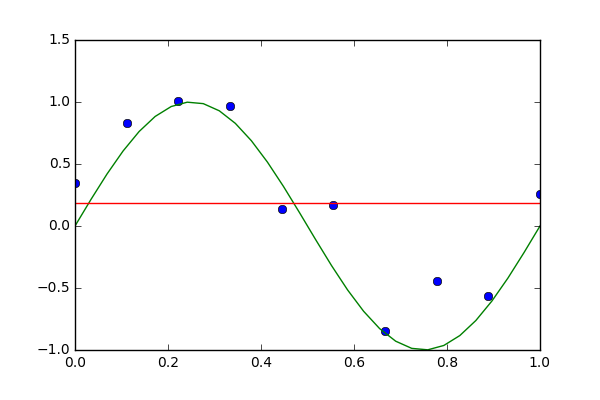
\includegraphics[width=4.3cm]{../Figures/Q2/M0.png}
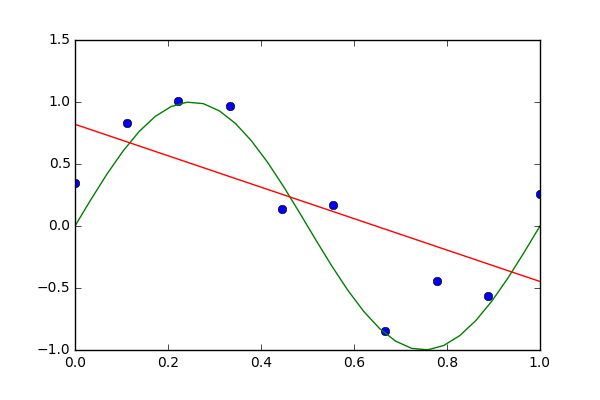
\includegraphics[width=4.3cm]{../Figures/Q2/M1.png}
 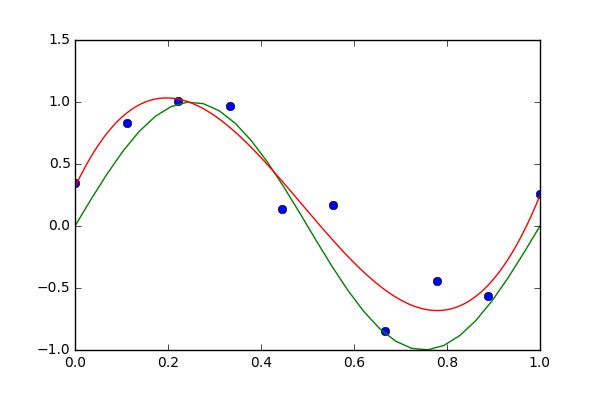
\includegraphics[width=4.3cm]{../Figures/Q2/M3.png}
 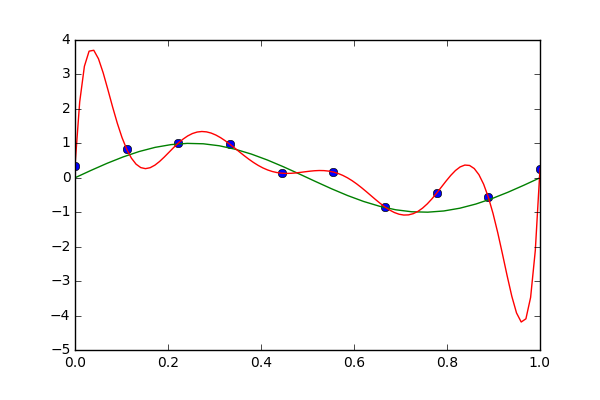
\includegraphics[width=4.3cm]{../Figures/Q2/M9.png}
\caption{Figures obtained using the optimal $w$ from {\tt regressionFit}}
\label{Bishop}
\end{figure}

\subsection{Sum of Squared Errors}
Using the notation for all $i \in [0,N-1]$, $Y_{pred}[i] = \sum_{j = 0}^M w_j X[i]^j$, we wrote a function {\tt sse } that leveraged the identity:
$$SSE = \sum_{i = 0}^{N-1} (Y_{pred}[i] - Y[i]) ^2.$$ 
And similarly, we wrote a function {\tt gradsse } based on the identity:
$$\frac{\partial SSE}{\partial w_j} = -2 \sum_{i = 0}^{N-1} X[i]^j (Y_{pred}[i] - Y[i]).$$ 

We verified the value of the gradient of the SSE function using the {\tt numericalGradient} function obtained in section \ref{numGrad}. We did our test with $M = 3$, for a variety of values for $w$. We used  {\tt numericalGradient} with $\eta = 0.01$. As we see in the following table, the numerical approximation of $(\nabla SSE) (w)$ and the closed form solution yield the same results with precision $0.1$. 

\begin{center}
  \begin{tabular}{| c  | c |c |}
    \hline
 $w$ & $(\nabla SSE) (w)$ &  $(\nabla_{num}SSE)(w)$ \\ \hline
 (2,2,2,2)  &  (81.46,  55.25,  43.89,  37.02) & (81.56,  55.29,  43.91 ,  37.04) \\ \hline
(1,2,0,-1) &  (30.72,  20.12,  15.23,  12.24)  & (30.82,  20.15,  15.25,  12.25) \\ \hline
(5,2,-4,0) & (88.13,  42.57,  28.77,  21.77) & (88.23,  42.61,  28.79,  21.79) \\
    \hline
  \end{tabular}
\end{center}

\subsection{Gradient Descent to optimize SSE}
For $M = 0, 1, 3$ the gradient descent algorithm converges for any initial point we tried, for a step size small enough. However, for $M=9$, and "reasonable" $x_0$, the algorithm does not converge towards the global minimum (as can be seen in figure \ref{Bishop}) but rather to an interpolation that looks very similar to the case $M=3$. The optimal case can be obtained by starting close to the solution $w \approx (  0.34, 2.3*10^2,  -5.3*10^3,   4.8*10^4,  -2.3*10^5,   6.4*10^5,  -1.1*10^6,   1.0*10^6, -5.6*10^5,   1.3*10^5)$.
\begin{figure}[h!]
  \centering
 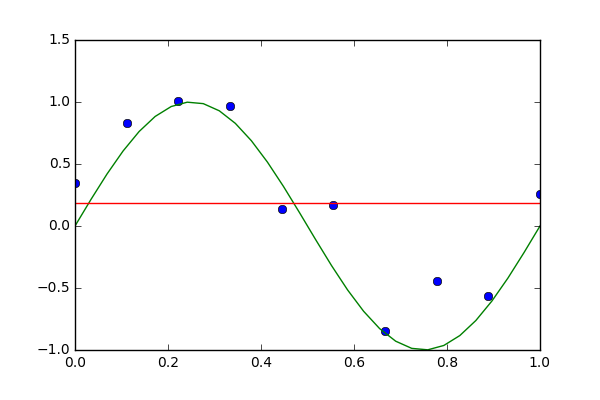
\includegraphics[width=4.3cm]{../Figures/Q2/M0bis.png}
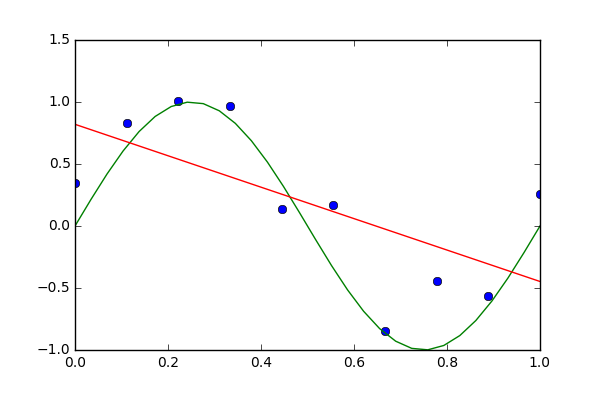
\includegraphics[width=4.3cm]{../Figures/Q2/M1bis.png}
 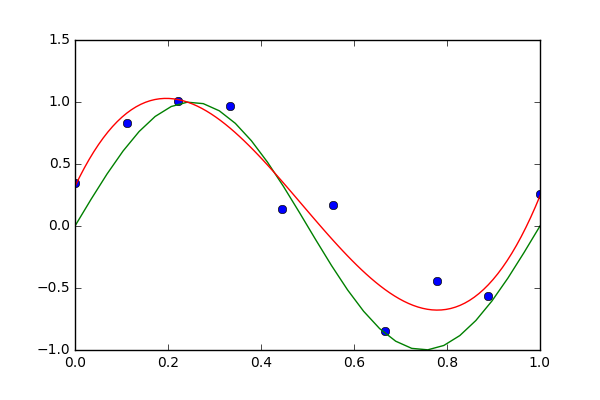
\includegraphics[width=4.3cm]{../Figures/Q2/M3bis.png}
 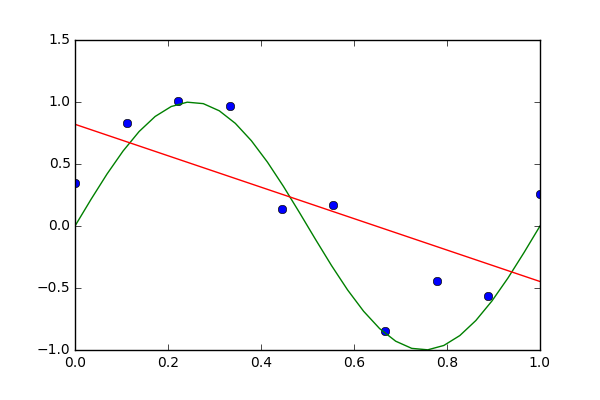
\includegraphics[width=4.3cm]{../Figures/Q2/M9quat.png}
\caption{Figures obtained using the $w$ computed using from {\tt gradientDescent} to minimize the SSE. $w = 0 \in \mathbb{R}^10$, $s= 0.04$ and $\epsilon = 10^{-7}$.}
\label{Bishop}
\end{figure}

This shows that the optimal interpolation polynomial is only one of the many local minima of the SSE function.

We next compare the number of calls to SSE needed by {\tt gradientDescent} and {\tt scipy.optimize.fmin\_bfgs} to achieve a precision of $\epsilon = 10^{-9}$.
\begin{center}
  \begin{tabular}{| c  | r |r |r |r |}
    \hline
 M & iterations {\tt GD} & iterations  {\tt bfgs} & error {\tt GD} & error  {\tt bgfs}  \\ \hline
 $0$ & $14$  & $3$ & $3.77$ & $3.77$ \\ \hline
 $1$ & $232$ &$5$ & $2.13$ & $2.13$ \\ \hline
 $3$ & $45906$ & $15$ & $0.35$ & $0.35$\\ \hline
  $9$ & $\geq 300,000$ &  $205$ & $0.34$ & $0.079$ \\
    \hline
  \end{tabular}
\end{center}


\subsection{Sin basis functions}
If we use sin basis functions, the optimal function is always very close to the original sin function. However, if we didn't know the original data was generated by a sin function, this could prevent us from reaching the optimal function. For instance all linear combinations of sin functions will have value 0 at 0. Therefore if our original functions was non-zero at the origin, it can never be obtained with sin functions.